\section{Dynamic-MSV-Bench and Methodology}
\label{sec:benchmark}

We propose the \textbf{Dynamic-MSV-Bench}, which categorizes multi-shot prompts into two extreme stress-test scenarios to expose the "Double-Kill" dilemma of current models.

\begin{figure*}[ht]
    \centering
    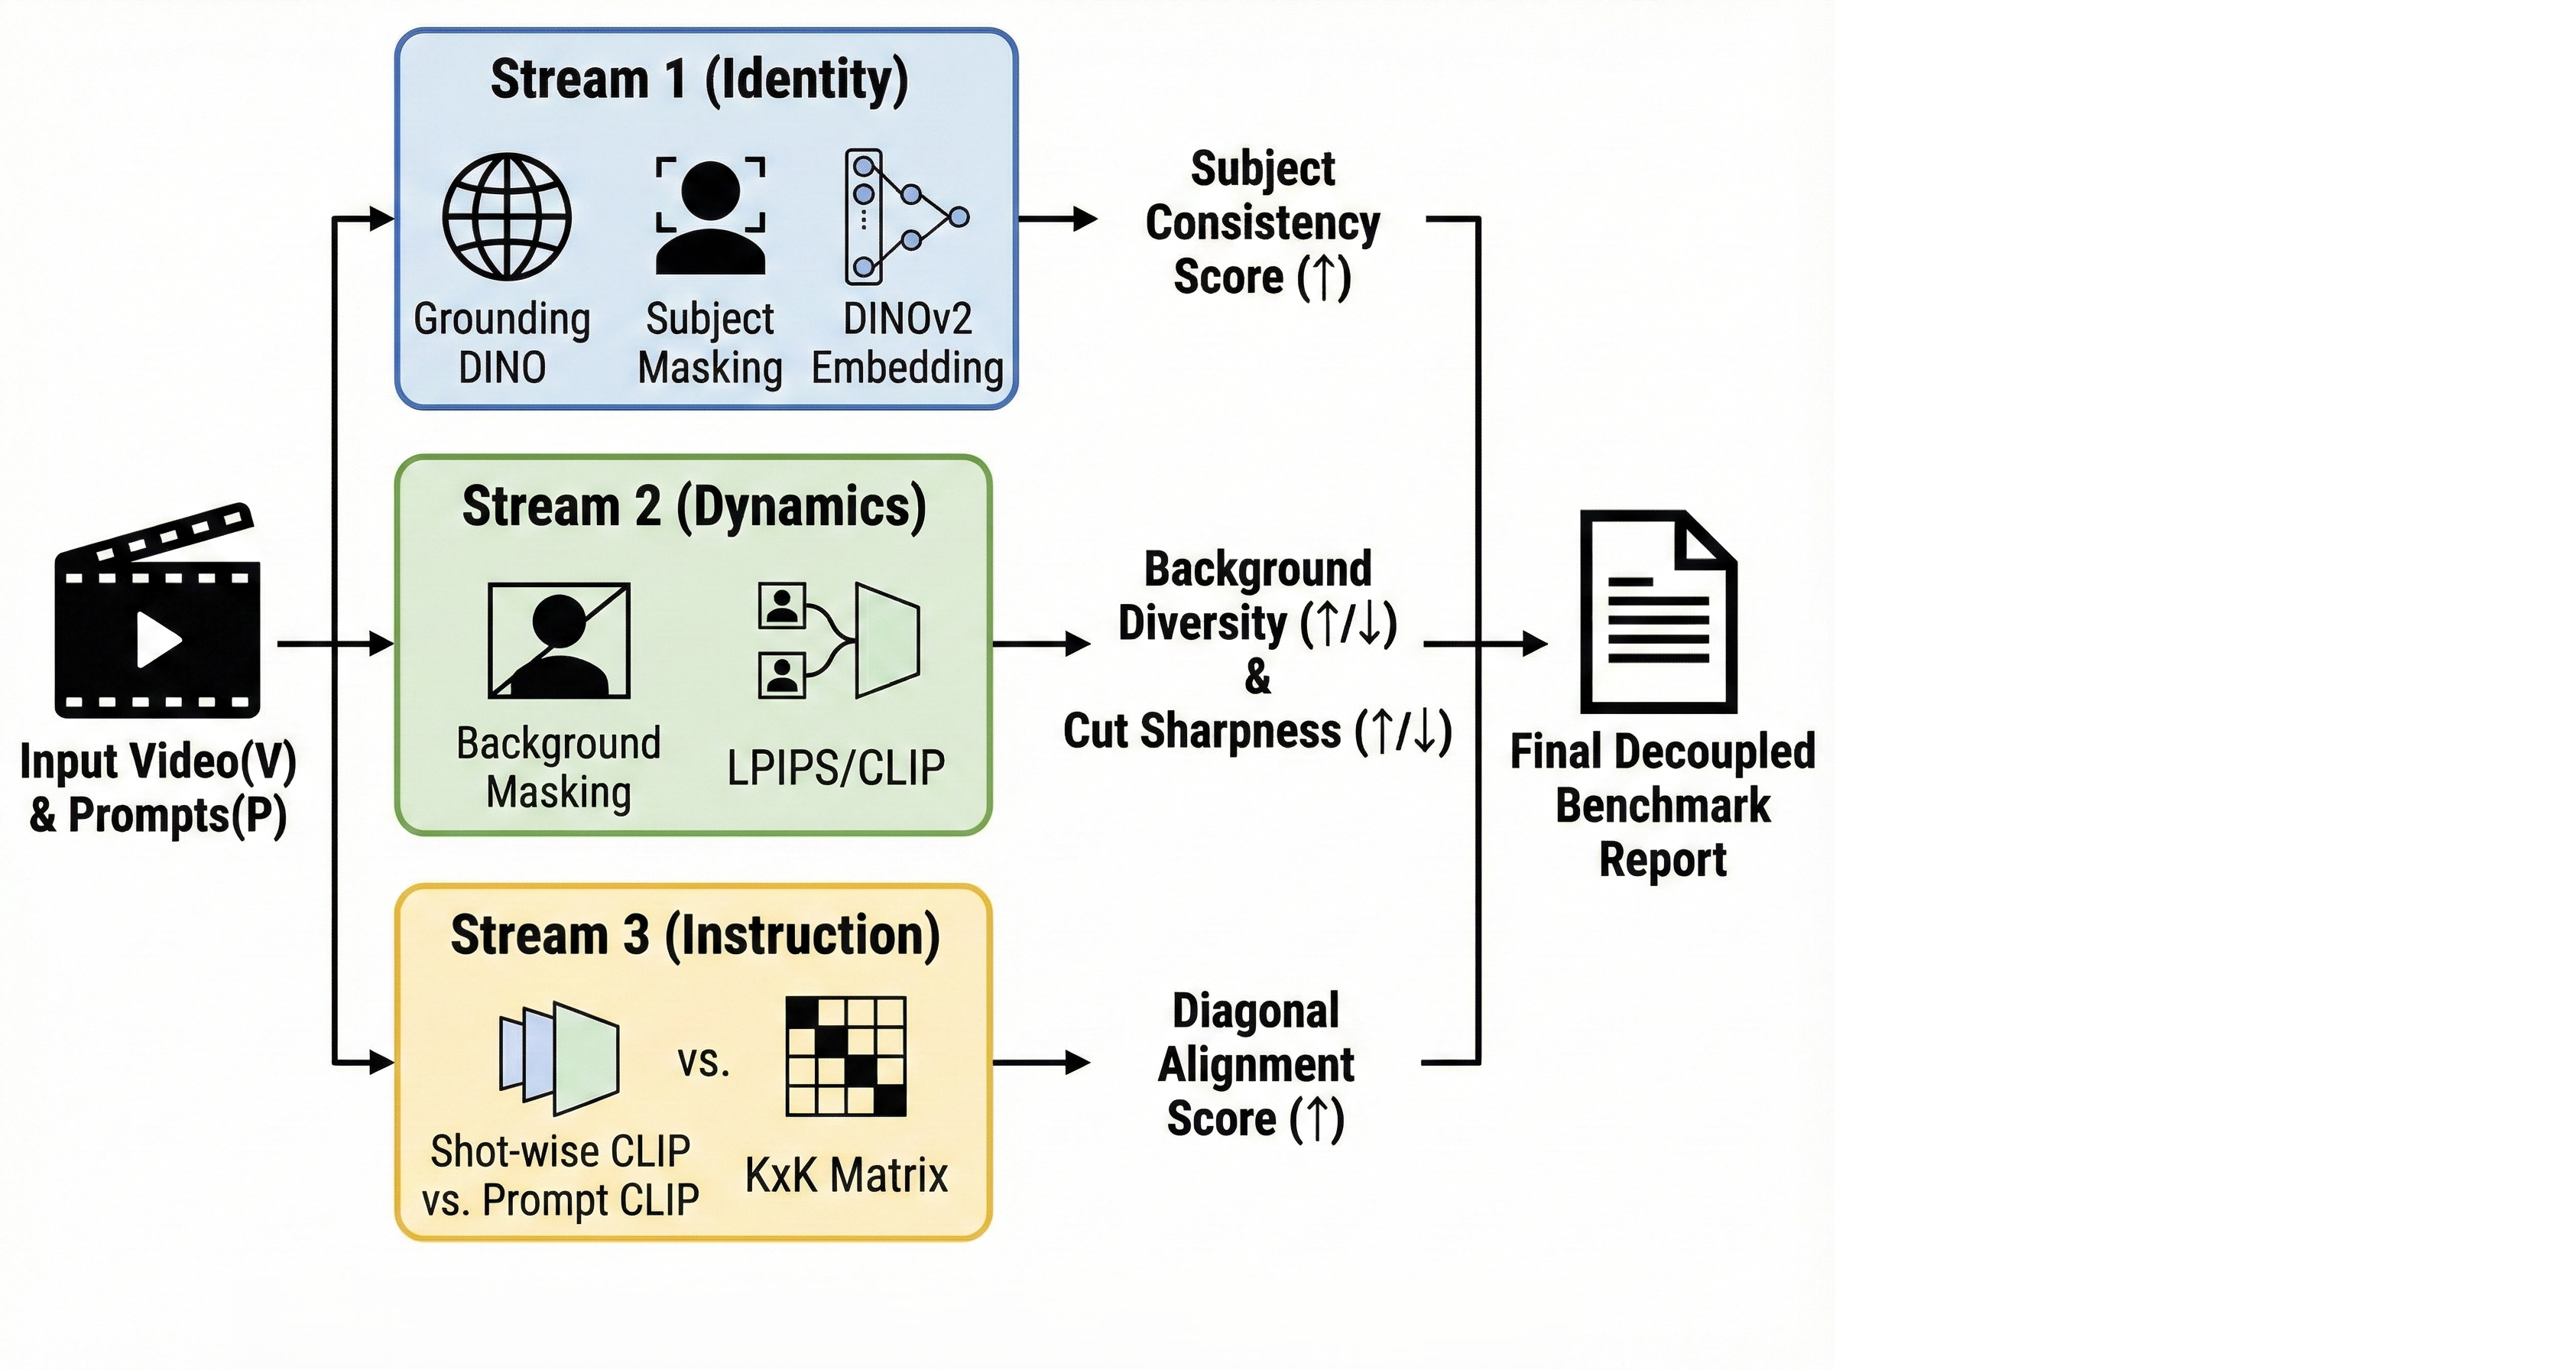
\includegraphics[width=\textwidth]{figures/fig2.jpg}
    \caption{Overview of our Decoupled 4D Evaluation Framework. Unlike holistic metrics like FVD, we process the input video through three independent streams to measure Subject Identity, Background Dynamics/Continuity, and Instruction Following (Diagonal Alignment) separately.}
    \label{fig:framework}
\end{figure*}

\begin{figure*}[ht]
    \centering
    \includegraphics[width=\textwidth]{figures/fig_AB.jpg}
    \caption{Conceptual comparison of our two evaluation tracks. (Left) \textbf{Track S: Semantic Leap} tests narrative diversity, requiring radical environment changes while preserving the subject. This track demands high Background Diversity and sharp cinematic cuts. (Right) \textbf{Track M: Motion Continuity} evaluates spatial integrity, where the background must remain consistent while the camera executes specific motions (Panning, Zooming, Tracking). Set M rewards low diversity and smooth spatial continuity.}
    \label{fig:sets_comparison}
\end{figure*}

\subsection{Track S: Semantic Leap (Narrative Diversity)}
Track S evaluates the model's ability to maintain a consistent subject while drastically shifting the semantic environment. 
The \textbf{Golden Rule for Track S} is defined as HIGH Background Diversity ($\uparrow$), HIGH Cut Sharpness ($\uparrow$), and HIGH Subject Consistency ($\uparrow$). 
\begin{itemize}
    \item \textbf{Background Diversity ($\uparrow$):} Since the narrative requires a leap between disparate locations (e.g., from a dense forest to outer space), the model must exhibit high variance in its environmental rendering. A low score here directly exposes the \textit{Static Trap}, where the model fails to transition despite the prompt.
    \item \textbf{Cut Sharpness ($\uparrow$):} These environmental jumps should be depicted as distinct cinematic cuts. High sharpness at the shot boundaries ensures that the scenes are rendered independently, without "morphing" artifacts where one location slowly dissolves into another.
    \item \textbf{Subject Consistency ($\uparrow$):} Despite the radical background changes, the identity of the main protagonist must remain strictly preserved to maintain narrative logic across the leap.
\end{itemize}

\subsection{Track M: Motion Continuity (Spatial Integrity)}
Track M tests physical instructions while keeping the background stable. 
The \textbf{Golden Rule for Track M} is defined as LOW Background Diversity ($\downarrow$), LOW Cut Sharpness ($\downarrow$), and HIGH Subject Consistency ($\uparrow$).
\begin{itemize}
    \item \textbf{Background Diversity ($\downarrow$):} The background environment must remain pixel-consistent while the camera moves. In this track, high diversity is a failure mode indicating \textit{Background Hallucination}, where the model cannot maintain spatial integrity during motion.
    \item \textbf{Cut Sharpness ($\downarrow$):} Unlike the narrative cuts in Track S, transitions between camera actions (e.g., from panning to zooming) should be spatially continuous. Low sharpness at the boundary rewards the model's ability to maintain a single, cohesive 3D space during physical camera transitions.
    \item \textbf{Subject Consistency ($\uparrow$):} The protagonist must be preserved throughout the camera actions, ensuring the motion is perceived as a change in perspective rather than an identity shift.
\end{itemize}

\subsection{The 4D Decoupled Metrics}
Our framework utilizes four indices:
\begin{enumerate}
    \item \textbf{Subject Consistency ($\mathcal{C}_{subj}$):} DINOv2~\cite{oquab2023dinov2} similarity of masked subject regions across $K$ shots.
    \item \textbf{Background Diversity ($\mathcal{D}_{bg}$):} Variance of CLIP/DINO embeddings in the environment region.
    \item \textbf{Cut-Transition Sharpness ($\mathcal{S}_{cut}$):} Normalized LPIPS~\cite{zhang2018perceptual} distance peaks at shot boundaries.
    \item \textbf{Diagonal Semantic Alignment (DSA):}
    Our core novelty, DSA, uses column-wise softmax probabilities:
    $$P_{i,j} = \frac{\exp(\tau \cdot M_{i,j})}{\sum_{k=1}^{K} \exp(\tau \cdot M_{k,j})}$$
    $$DSA = \frac{\left( \frac{1}{K} \sum_{i=1}^{K} P_{i,i} \right) - \frac{1}{K}}{1 - \frac{1}{K}}$$
    This formulation ensures that a static video yields a DSA of exactly 0.0.
\end{enumerate}
